\chapter{Results}
This work's implementation of the proposed platform is described in section \ref{sec:proposed-platform-implementation}. Its performance metrics, such as its latency, throughput, power, and energy consumption, are compared to the available alternative technologies and FPGA architectures. AlexNet is the selected CNN to be used as a benchmark for the various technologies compared.

\section{Specifications of the Compared Platforms}
The proposed platform is compared with an Intel i7 4710MQ CPU, an NVIDIA RTX 2060 Super 8GB GPU, a Xilinx CHaiDNN implementation, and a Xilinx DPU implementation. All FPGA implementations, including this work's platform, use the Xilinx ZCU102 Evaluation board.

% \subsection{AMD Ryzen 5 1400}
% The AMD Ryzen 5 1400 CPU \cite{AMD-Ryzen-5-1400-Processor}, released in 2017, is a desktop processor targeted for mid-range productivity computers. Its specifications are presented in table \ref{tab:AMD-Ryzen-5-1400-specs}.

% \begin{table}[H]
% 	\caption{AMD Ryzen 5 1400 processor specifications}
% 	\label{tab:AMD-Ryzen-5-1400-specs}
% 	\centering
% 	\begin{tabular}{ll}
% 		\toprule
% 		\textbf{Cores / Threads} & 4/8\\
% 		\textbf{Max Turbo Frequency} & 3.4GHz\\
% 		\textbf{TDP} & 65W\\
% 		\textbf{Max Memory Bandwidth} & 42.7GB/s\\
% 		\textbf{Lithography} & 14nm\\
% 		\bottomrule
% 	\end{tabular}
% \end{table}

\subsection{Intel i7 4710MQ}
The Intel i7 4710MQ CPU \cite{Intel-i7-4710MQ-Processor}, released in 2014, is a mobile processor targeted for high-performance laptops. Its specifications are presented in table \ref{tab:Intel-i7-4710MQ-specs}.

\begin{table}[H]
	\caption{Intel i7 4710MQ processor specifications}
	\label{tab:Intel-i7-4710MQ-specs}
	\centering
	\begin{tabular}{ll}
		\toprule
		\textbf{Cores / Threads} & 4/8\\
		\textbf{Max Turbo Frequency} & 3.5GHz\\
		\textbf{TDP} & 47W\\
		\textbf{Max Memory Bandwidth} & 25.6GB/s\\
		\textbf{Lithography} & 22nm\\
		\bottomrule
	\end{tabular}
\end{table}

\subsection{NVIDIA RTX-2060 Super 8GB}
The NVIDIA RTX-2060 Super \cite{NVIDIA-RTX-2060-Super}, released in 2019, is a desktop GPU, and while targeted for raytraced gaming, it is also suitable for CNN inferencing due to its large and high-bandwidth memory. Its specifications are presented in table \ref{tab:NVIDIA-RTX-2060-Super-specs}.

\begin{table}[H]
	\caption{NVIDIA RTX 2060 Super specifications}
	\label{tab:NVIDIA-RTX-2060-Super-specs}
	\centering
	\begin{tabular}{ll}
		\toprule
		\textbf{CUDA Cores} & 2176\\
		\textbf{GPU Memory} & 8GB GDDR6\\
		\textbf{Boost Clock} & 1650 MHz\\
		\textbf{Memory Interface} & 256-bit\\
		\textbf{Memory Bandwidth} & 448GB/s\\
		\textbf{Power Consumption} & 175W\\
		\bottomrule
	\end{tabular}
\end{table}

\subsection{Xilinx CHaiDNN}
The Xilinx CHaiDNN accelerator library, presented in section \ref{sec:Xilinx-CHaiDNN}, was implemented for this work's comparisons. The resource utilization for its implementation is depicted in table \ref{tab:CHaiDNN-resource-usage}. It should be noted that Double Pumped DSPs are used.

\begin{table}[H]
	\caption{Xilinx CHaiDNN resource usage}
	\label{tab:CHaiDNN-resource-usage}
	\centering
	\begin{tabular}{ll}
		\toprule
		\textbf{PL/DSP Clock Frequency} & 250/500 MHz\\
		\textbf{LUT Usage} & 59.1\%\\
		\textbf{LUTRAM Usage} & -\\
		\textbf{FF Usage} & 27.66\%\\
		\textbf{BRAM Usage} & 74.12\%\\
		\textbf{DSP Usage} & 53.65\%\\
		\textbf{BUFG Usage} & -\\
		\bottomrule
	\end{tabular}
\end{table}

% \subsection{Xilinx DPU}
% The Xilinx DPU accelerator library, presented in section \ref{sec:Xilinx-DPU}, was implemented for this work's comparisons. The resource utilization for its implementation is depicted in table \ref{tab:DPU-resource-usage}.

% \begin{table}[H]
% 	\caption{Xilinx DPU resource usage}
% 	\label{tab:DPU-resource-usage}
% 	\centering
% 	\begin{tabular}{ll}
% 		\toprule
% 		\textbf{Clock Frequency (MHz)} & 300/600\\
% 		\textbf{LUT Usage (\%)} & 7.34\\
% 		\textbf{LUTRAM Usage (\%)} & 2.05\\
% 		\textbf{FF Usage (\%)} & 4.03\\
% 		\textbf{BRAM Usage (\%)} & 7.51\\
% 		\textbf{DSP Usage (\%)} & 1.9\\
% 		\textbf{BUFG (\%)} & 0.25\\
% 		\bottomrule
% 	\end{tabular}
% \end{table}

\section{Proposed Platform}
\label{sec:proposed-platform-implementation}
This work's proposed platform can be implemented using several data types and accelerators. For this comparison, it was implemented based on AlexNet's requirements and characteristics, presented in chapter \ref{Chapter-Theoretical-Modeling-and-Robustness-Analysis}. Both parameters and activations are represented as 8-bit fixed-points; hence, the accelerators use the same data type. There is a single accelerator instance per layer type, using their high-performance versions as presented in section \ref{sec:Platform-Accelerator-Architectures}. The serial execution scheduler (see section \ref{sec:Scheduler-Strategies}) was selected because the implemented accelerators do not support layer pipelining, and there are not multiple instances per layer type.

The resource utilization for implementing the aforementioned configuration of the proposed platform is depicted in table \ref{tab:Proposed-platform-resource-usage}.

\begin{table}[H]
	\caption{Proposed platform resource usage}
	\label{tab:Proposed-platform-resource-usage}
	\centering
	\begin{tabular}{ll}
		\toprule
		\textbf{Clock Frequency (MHz)} & 300MHz\\
		\textbf{LUT Usage} & 7.34\%\\
		\textbf{LUTRAM Usage} & 2.05\%\\
		\textbf{FF Usage} & 4.03\%\\
		\textbf{BRAM Usage} & 7.51\%\\
		\textbf{DSP Usage} & 1.9\%\\
		\textbf{BUFG (\%)} & 0.25\%\\
		\bottomrule
	\end{tabular}
\end{table}

\section{Performance Metrics}
\subsection{Throughput}
Throughput, defined in equation \ref{eqn:throughput}, is the number of tasks that can be accomplished in a unit time. It is preferred to be as high as possible to generate as much work as possible in the unit time.

\subsection{Latency}
Latency, defined in equation \ref{eqn:latency}, is the time required for accomplishing a single task. It is preferred to be as low as possible to finish tasks as quickly as possible from the time they are issued.

\subsection{Power Consumption}
Power consumption is defined as the energy consumed per unit time for accomplishing a specific task, from a chemical reaction and lifting materials using a crane, to emitting light through a light bulb and inferencing CNNs on electronic hardware. Average power consumption is always preferred to be as low as possible to increase the system's energy efficiency, minimizing energy losses. In addition, low power consumption leads to simpler system designs and lower building costs. It is usually measured in Watts (w) or kiloWatts (kW).

\subsection{Energy Consumption}
Energy consumption is defined as the energy required for accomplishing a specific task in a specific time amount. It can be calculated as $Energy = Power * Time$, where $Power$ is the required power, and $Time$ is the required time for accomplishing the task. Energy consumption is also preferred to be as low as possible while accomplishing the given task within the time constraints, to minimize the operational costs. It is usually measured in Joule (J) or kiloJoule (kJ).

\section{CPU and GPU Performance}
PyTorch provides the option to select the appropriate input batch size that best suits the application's needs concerning the hardware in use. Every CPU and GPU has different architecture and configuration, and, consequently, the best batch size can vary. In general, larger batch sizes increase both inference throughput and latency. However, very large batch sizes can damage the application's throughput. Hence, a low-latency application should use small batch sizes but expect lower throughput, and high-throughput applications should use large batch sizes with higher latency costs.

A Python script was created to measure the CPU and GPU inference performance regarding the selected batch size. The script uses the prebuilt and pre-trained AlexNet model provided by PyTorch and tests the performance using all the available batch sizes. Figure \ref{fig:CPU-vs-GPU-Inference-Latency} depicts the inference latency on both platforms in milliseconds per image.

\begin{figure} [H]
	\centering
	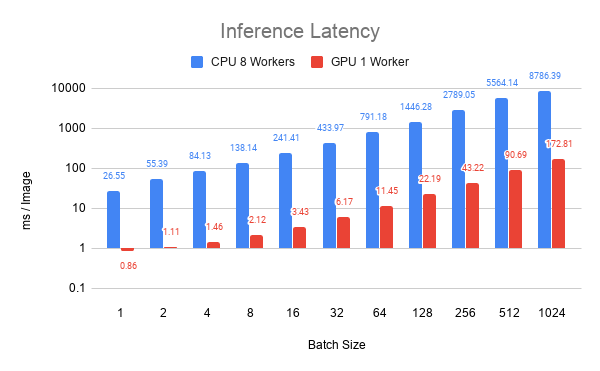
\includegraphics[width=\textwidth]{Images/Results/CPU-GPU-Inference-Latency.png}
	\decoRule
	\caption[CPU vs GPU Inference Latency]{CPU vs GPU Inference Latency: Latency increases while batch size increases on both platforms.}
	\label{fig:CPU-vs-GPU-Inference-Latency}
\end{figure}

As expected, the latency increases while the batch size increases. It is remarkable that the GPU achieves almost two orders of magnitude lower latency than the CPU on all batch sizes.

Figure \ref{fig:CPU-vs-GPU-Inference-Throughput} depicts the inference throughput on both platforms in images per second. While the CPU's throughput increases as the batch size increases, the GPU's throughput reaches its maximum on 256 batch size, and from then on, it decreases. Almost two orders of magnitude difference between the two platforms are also appearing.

\begin{figure} [H]
	\centering
	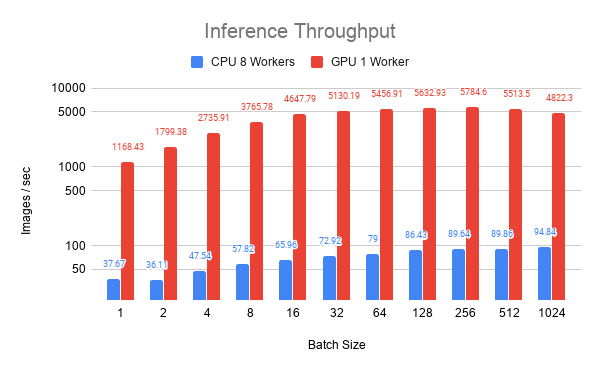
\includegraphics[width=\textwidth]{Images/Results/CPU-GPU-Inference-Throughput.png}
	\decoRule
	\caption[CPU vs GPU Inference Throughput]{CPU vs GPU Inference Throughput: Throughput increases while batch size increases on CPU, while the GPU reaches its maximum throughput on 256 batch size.}
	\label{fig:CPU-vs-GPU-Inference-Throughput}
\end{figure}

It should be noted that PyTorch also can configure the number of workers to be used for its inference procedure. A worker can be thought of as an orchestrator, processes that run in parallel to inference images. As a rule of thumb, which has also been tested but not shown on the previous figures, it is best to use the same amount of workers as the number of available threads in a CPU. A single worker should also be used when inferencing with a GPU because multiple workers can create communication bottlenecks and damage performance. Therefore, the aforementioned tests were conducted using eight workers when inferencing on the CPU, and a single worker when inferencing on the GPU.

\section{Final Performance}
The comparisons were conducted using the same dataset and AlexNet hyper-parameters across all technologies. The CPU and GPU use floating-point arithmetic for their parameters and activations, while CHaiDNN uses 8-bit quantization, and the proposed platform implementation uses 8-bit fixed-point arithmetic.

Table \ref{tab:Performance-results} depicts the comparison results of every technology. It should be noted that the CPU and GPU use different batch sizes for their throughput and latency measurements to represent their best performance. In this case, the CPU uses a batch size of 1024 for throughput and a batch size of 1 for latency, and the GPU uses a batch size of 256 for throughput and a batch size of 1 for latency.

The Energy Consumption/Image metric is calculated as shown on equation \ref{eqn:joule-per-image}.
\begin{equation}
	\label{eqn:joule-per-image}
	\frac{Energy Consumption}{Image} = \min \{TotalPower * Latency, \frac{TotalPower}{Throughput}\}
\end{equation}

The Images/Joule metric is calculated, as shown in equation \ref{eqn:images-per-joule}.
\begin{equation}
	\label{eqn:images-per-joule}
	\frac{Images}{Joule} = \max \{\frac{1}{TotalPower * Latency}, \frac{Throughput}{TotalPower}\}
\end{equation}

The throughput and latency speedups, and the power and energy efficiencies for every platform are calculated compared to the CPU.

\begin{table}[H]
	\caption{Performance results}
	\label{tab:Performance-results}
	\centering
	\begin{tabular}{l|l|l|l|p{2cm}}
		\toprule
		& \textbf{CPU} & \textbf{GPU} & \textbf{CHaiDNN} & \textbf{Proposed Platform}\\
		\midrule
			\textbf{Clock Frequency (MHz)} & 3500 & 1650 & 250/500 & 300\\
			\textbf{Throughput (Images/s)} & 94.84 & 5784.6 & 10.07 & 0.0927\\
			\textbf{Throughput Speedup} & 1x & 60.9933x & 0.1062x & 0.001x\\
			\textbf{Latency (s)} & 0.0266 & 0.0009 & 0.0993 & 10.783\\
			\textbf{Latency Speedup} & 1x & 29.5556x & 0.2679x & 0.0025x\\
			\textbf{Total On-Chip Power (Watt)} & 47 & 175 & 19.3 & 4.559\\
			\textbf{Power Efficiency} & 1x & 0.2686x & 2.4352x & 10.3093x\\
			\textbf{Energy Cons./Image (Joule)} & 1.2502 & 0.1575 & 1.9165 & 49.1597\\
			\textbf{Energy Efficiency} & 1x & 7.9378x & 0.6523x & 0.0254x\\
			\textbf{Images/Joule} & 2.0179 & 33.0549 & 0.5218 & 0.0203\\
		\bottomrule
	\end{tabular}
\end{table}

The final results of the various performance metrics are also depicted using bar charts in figure \ref{fig:Final-Results-charts} for better visibility.

\begin{figure} [H]
	\centering
	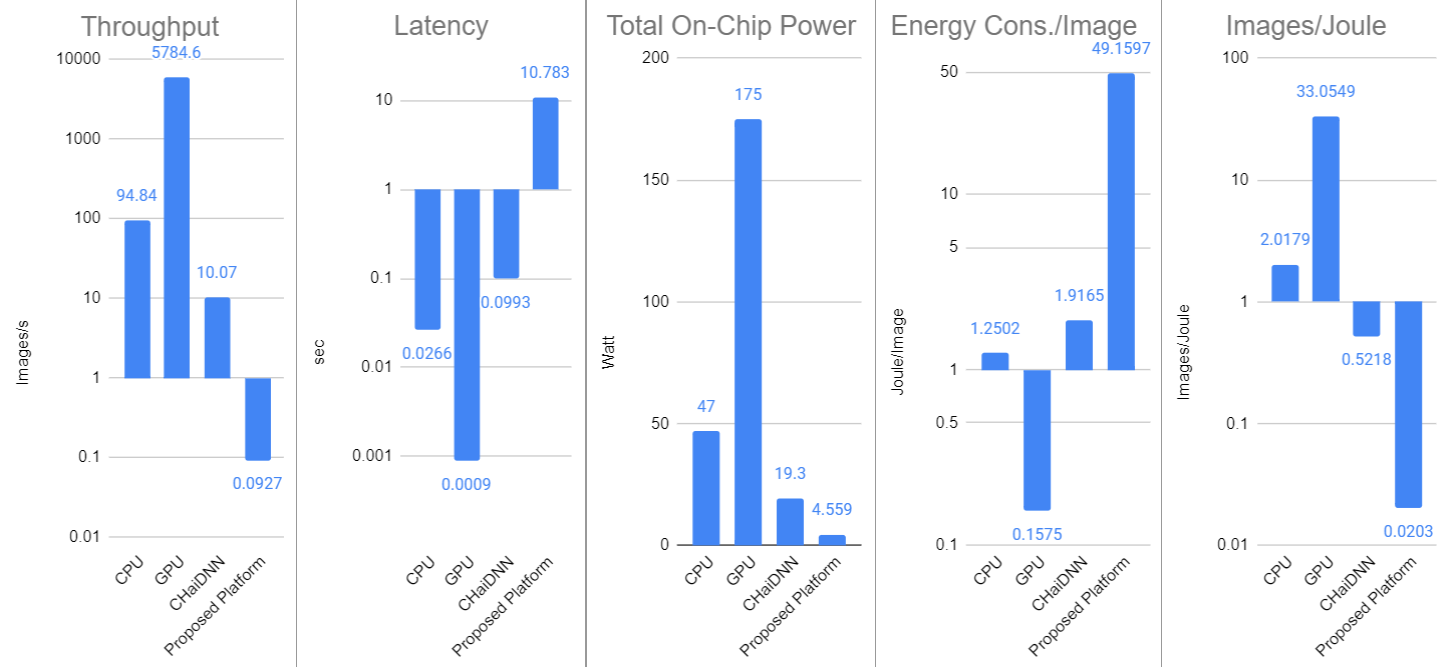
\includegraphics[width=\textwidth]{Images/Results/Final-Results-charts.png}
	\decoRule
	\caption[Final Results Charts]{Final Results Charts: While requiring the highest amount of power, the GPU stands out in every other performance metric.}
	\label{fig:Final-Results-charts}
\end{figure}

It can be observed that while the GPU in use requires almost four times the power of its CPU counterpart, it can provide the best performance in every metric, with an almost 61 times throughput speedup and an almost 30 times latency speedup. Although the GPU is the most power-hungry device, it achieves the energy efficiency across all platforms due to its low latency and high throughput capabilities.

Both tested FPGA platforms, the CHaiDNN and the proposed platform, have worse results in every metric compared to the CPU and GPU. However, CHaiDNN and the proposed platform beat their counterparts with more than 2 times and 10 times lower power requirements, respectively. Between the two FPGA platforms, CHaiDNN performs better in terms of throughput, latency, and energy consumption, but requires more than 4 times the proposed platform's power and much more hardware resources, as shown in tables \ref{tab:CHaiDNN-resource-usage} and \ref{tab:Proposed-platform-resource-usage}.

Although the proposed platform's performance is lower than expected for a real-world application, this significant difference in resource utilization between the two platforms creates an opportunity for further development to achieve better results. The priority for further development should be given to the Convolution accelerator, which consumed about 98\% of the total inference time in the tests. First of all, the Double-Pumped DSPs technique used by both Xilinx CHaiDNN and Xilinx DPU should also be used by the proposed platform to create a speedup of up to 2 times. Secondly, the convolution algorithm should be further unrolled to convolve in a single clock cycle the whole kernel, not just row-by-row like the convolution accelerator shown in figure \ref{fig:conv-core-row-parallel}, or even multiple kernels, striding from left to right. Furthermore, the Max-Pooling accelerator's functionality could be integrated into the Convolution accelerator, applying its operations after creating a single output channel and before the ReLU functionality. This way, the ReLU is also applied to fewer outputs due to the Max-Pooling's down-sampling nature. Additionally, communication is decreased because there is no need for the convolution results to be transferred to the Max-Pooling accelerator, either by MMIO or stream, since they are passed-through directly from the same BRAM instances. Finally, other architectures could also be designed, such as by incorporating a systolic array.
